\documentclass{beamer}


% For more themes, color themes and font themes, see:
% http://deic.uab.es/~iblanes/beamer_gallery/index_by_theme.html


\mode<presentation>
{
	\usetheme{Madrid}       % or try default, Darmstadt, Warsaw, ...
	\usecolortheme{wolverine} % or try albatross, beaver, crane, ...
	\usefonttheme{default}    % or try default, structurebold, ...
	\setbeamertemplate{navigation symbols}{}
	\setbeamertemplate{caption}[numbered]
} 

\usepackage{lmodern}
\usepackage[english]{babel}
\usepackage[utf8]{inputenc}
\usepackage{chemfig}
\usepackage[version=3]{mhchem}
\usepackage{amsmath}
\usepackage{mathtools}
\usepackage[absolute,overlay]{textpos}
\usepackage{graphicx}
\graphicspath{ {img/} }
\usepackage[absolute,overlay]{textpos}
\usepackage{bm}
\usepackage[normalem]{ulem}
\usepackage{cancel}
\usepackage{relsize}
\usepackage[export]{adjustbox}
\usepackage[T1]{fontenc}

\definecolor{ForestGreen}{rgb}{0.13, 0.55, 0.13}

\newcommand\norm[1]{\left\lVert#1\right\rVert}
\newcommand\red[1]{\textcolor{red}{\textbf{#1}}}
\newcommand\blue[1]{\textcolor{blue}{\textbf{#1}}}
\newcommand\yellow[1]{\textcolor{yellow}{\textbf{#1}}}
\newcommand\green[1]{\textcolor{ForestGreen}{\textbf{#1}}}
\DeclarePairedDelimiterX{\ip}[2]{\langle}{\rangle}{#1, #2}
\DeclareMathOperator*{\argmax}{\arg\!\max}

% On Overleaf, these lines give you sharper preview images.
% You might want to `comment them out before you export, though.
\usepackage{pgfpages}
\pgfpagesuselayout{resize to}[physical paper width=8in, physical paper height=6in]

% Here's where the presentation starts, with the info for the title slide
\title[Joint Training of CNN and PGM for HPE]{\textbf{Joint Training of a Convolutional Network and a Graphical Model for Human Pose Estimation}}
\subtitle{}
\author{Y. Fan \& M. Andriushchenko}
\institute{Saarland Univ.}
\date{30 January 2018}

\begin{document}
	
	% Title page
	\begin{frame}
		\titlepage
	\end{frame}

    \begin{frame}[t]
        \frametitle{What is state-of-the-art in \textbf{human pose estimation}?}
        \begin{center}
            We all know that CNNs show state-of-the-art in many computer vision tasks. \\
            But what about PGMs? Do we actually need them?
        \end{center}
    \end{frame}





	\begin{frame}[t]
        \frametitle{Higher-Level Spatial Model}
        \begin{center}
            Problem: Part Detector produces many false-positives. \newline \newline
			Solution: use a Spatial Model to enforce the consistency.\\
        \end{center}
         \begin{figure}[htbp] % htbp stand for "here", "top", "bottom", "page"
            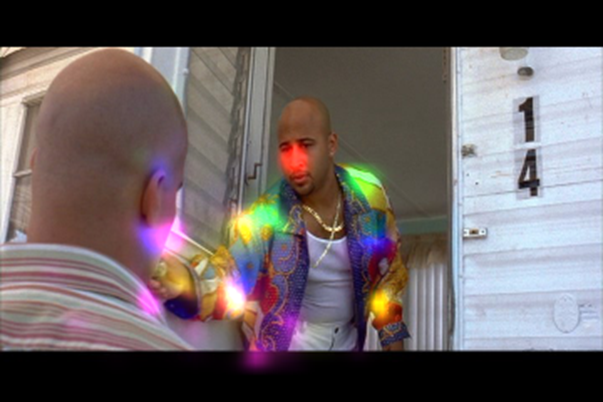
\includegraphics[scale=0.55]{false_positive.png}
         \end{figure}
    \end{frame}

	\begin{frame}[t]
        \frametitle{Spatial Model as a PGM}
        \begin{center}
			We adopt the star model.\\
            \begin{figure}[htbp] % htbp stand for "here", "top", "bottom", "page"
            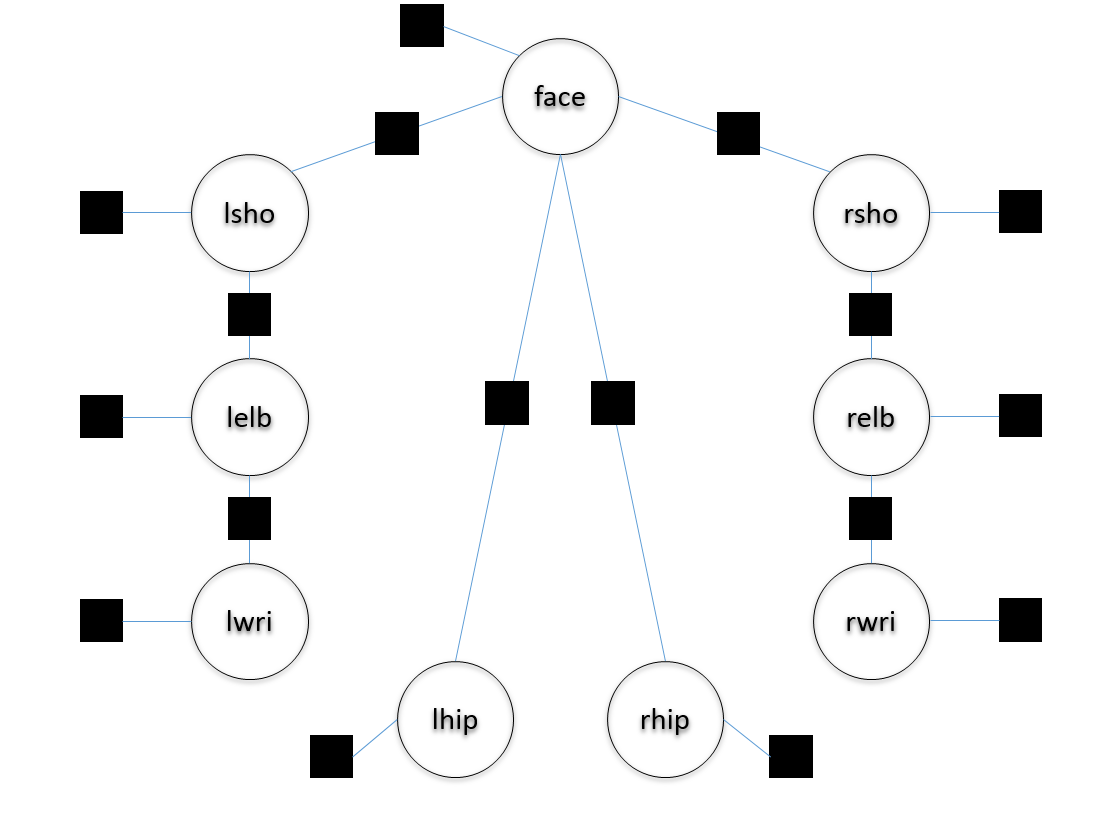
\includegraphics[scale=0.3]{star_model.png}
            \end{figure}
        \end{center}
    \end{frame}

    \begin{frame}[t]
        \frametitle{Pairwise Potentials}
        \begin{center}
            \begin{figure}[htbp] % htbp stand for "here", "top", "bottom", "page"
            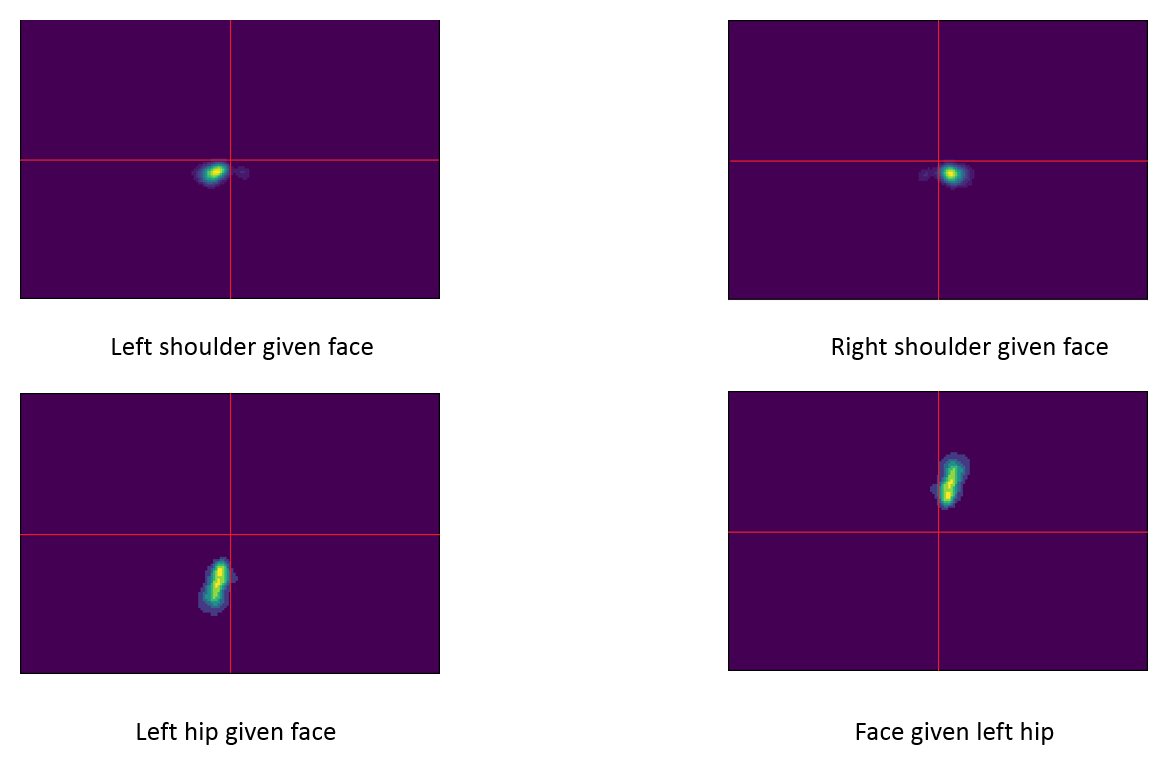
\includegraphics[scale=0.34]{pairwise_po.png}
            \end{figure}
        \end{center}
    \end{frame}

	\begin{frame}[t]
        \frametitle{Inference on PGM}
        \begin{center}
            %$\hat{p}_{i} \propto p_{i} \prod_{u\in U}(p_{i|u}*p_u)$ \\
            %where U is a set of neighbouring nodes of body part i
            \begin{figure}[htbp] % htbp stand for "here", "top", "bottom", "page"
            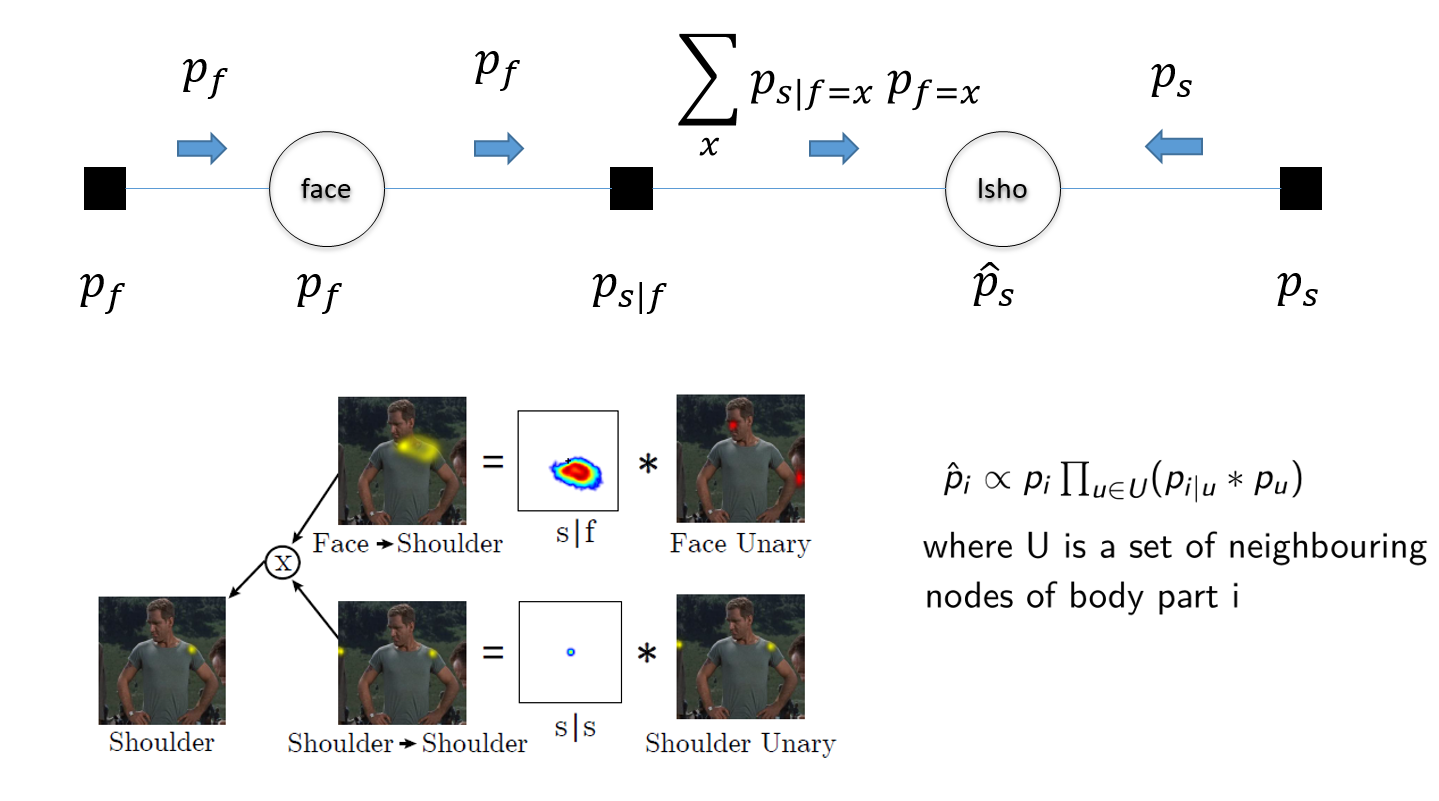
\includegraphics[scale=0.32]{inference.png}
            \end{figure}
        \end{center}
    \end{frame}

	\begin{frame}[t]
        \frametitle{Spatial Model as a trainable PGM}
        \begin{center}
            The Spatial Model can also be modeled as fully connected graph with trainable parameters.\newline \newline

        \end{center}

        \begin{flushleft}
            Star PGM:\\
            \begin{itemize}
                \item computationally efficient (during the train phase).\\
                \item Less parameters to be train.\\
                \item Inference is exact.\\
            \end{itemize}
            Fully Connected PGM:\\
            \begin{itemize}
                \item More model capacity.\\
                \item \textbf{The model is learned from the data, no need of expert prior.}\\
                \item Loopy structure has no guarantee of convergence.
            \end{itemize}
        \end{flushleft}
    \end{frame}



    \begin{frame}[t]
        \frametitle{Conclusions}
        \begin{itemize}
            \item We open sourced all our code in our Github repository: \url{https://github.com/max-andr/cnn_mrf_hybrid_for_hpe}! \\
            \item Up to our knowledge, this is the first implementation of the presented paper \cite{cnn_pgm_for_hpe}.
        \end{itemize}
    \end{frame}


	\begin{frame}[plain,c]
		%\frametitle{A first slide}
		\begin{center}
			\Huge \blue{Thanks for your attention!} \\ \ \\
			Any questions? \\
		\end{center}
	\end{frame}
	
	
	\section*{References}
	\begin{thebibliography}{}
		\setbeamertemplate{bibliography item}[text]
		
		\bibitem{cnn_pgm_for_hpe}
		\href{https://arxiv.org/abs/1406.2984}
		{Joint Training of a Convolutional Network and a Graphical Model for Human Pose Estimation}

		\bibitem{cnn_pgm_for_hpe}
		\href{https://arxiv.org/abs/1312.7302}
		{Learning Human Pose Estimation Features with Convolutional Networks}
	\end{thebibliography} 
\end{document}